%%%%%%%%%%%%%%%%%%%%%%%%%%%%%%%%%%%%%%%%%
% Journal Article
% LaTeX Template
% Version 1.3 (9/9/13)
%
% This template has been downloaded from:
% http://www.LaTeXTemplates.com
%
% Original author:
% Frits Wenneker (http://www.howtotex.com)
%
% License:
% CC BY-NC-SA 3.0 (http://creativecommons.org/licenses/by-nc-sa/3.0/)
%
%%%%%%%%%%%%%%%%%%%%%%%%%%%%%%%%%%%%%%%%%

% Editado por Mariela J. 04/02/2014
 
%----------------------------------------------------------------------------------------
%	PACKAGES AND OTHER DOCUMENT CONFIGURATIONS
%----------------------------------------------------------------------------------------

\documentclass[twoside]{article}

\usepackage[sc]{mathpazo} % Use the Palatino font
\usepackage[T1]{fontenc} % Use 8-bit encoding that has 256 glyphs
\linespread{1.05} % Line spacing - Palatino needs more space between lines
\usepackage{microtype} % Slightly tweak font spacing for aesthetics

%\usepackage[twoside,width=16cm,height=24cm,left=3cm]{geometry}
\usepackage[hmarginratio=1:1,top=20mm,width=19cm,height=23cm,columnsep=15pt]{geometry} % Document margins
\usepackage{multicol} % Used for the two-column layout of the document
\usepackage[hang, small,labelfont=bf,up,textfont=it,up]{caption} % Custom captions under/above floats in tables or figures
\usepackage{booktabs} % Horizontal rules in tables
\usepackage{float} % Required for tables and figures in the multi-column environment - they need to be placed in specific locations with the [H] (e.g. \begin{table}[H])
\usepackage{hyperref} % For hyperlinks in the PDF

%----------- Agregados para el caso de ustedes -------------------------------
\usepackage[spanish]{babel}% idioma castellano
\usepackage[utf8]{inputenc}% esto es para poder poner los tildes directamente. Puede que cambie de versión a versión de sistema operativos (más información en http://www.aq.upm.es/Departamentos/Fisica/agmartin/webpublico/latex/FAQ-CervanTeX/FAQ-CervanTeX-6.html )
\usepackage{graphicx} % para insertar figuras
\usepackage{subfigure} % para insertar figuras dentro de figuras
\usepackage{times} % plataforma
\usepackage{amsmath} % --para ecuaciones y algunos símbolos 
% ---------------------- -----------------------------------------------------

\usepackage{lettrine} % The lettrine is the first enlarged letter at the beginning of the text
\usepackage{paralist} % Used for the compactitem environment which makes bullet points with less space between them
\usepackage[T1]{fontenc}					%para poder usar tildes sin problemas

\usepackage{mathrsfs}
% Abreviaturas
\newcommand\CC{\mathbb{C}}
\newcommand\RR{\mathbb{R}}
\newcommand\QQ{\mathbb{Q}}
\newcommand\ZZ{\mathbb{Z}}
\newcommand\NN{\mathbb{N}}

\usepackage{abstract} % Allows abstract customization
\renewcommand{\abstractnamefont}{\normalfont\bfseries} % Set the "Abstract" text to bold
\renewcommand{\abstracttextfont}{\normalfont\small\itshape} % Set the abstract itself to small italic text
\addto\captionsspanish{ % Modifica algunos nombres cambiandolos por los definidos a continuacion
        \def\contentsname{\'Indice}%
        \def\bibname{Referencias}%
        \def\tablename{Tabla}%
        \def\abstractname{Resumen}
        }

\usepackage{titlesec} % Allows customization of titles
\usepackage{fancyhdr} % Headers and footers
\pagestyle{fancy} % All pages have headers and footers
\fancyhead{} % Blank out the default header
\fancyfoot{} % Blank out the default footer
\fancyhead[C]{Laboratorio 4 $\bullet$ 2017} % Custom header text
\fancyfoot[RO,LE]{\thepage} % Custom footer text

\providecommand{\dpart}[2]{\frac{\partial#1}{\partial#2}}
\providecommand{\dtot}[2]{\frac{\d#1}{\d#2}}
\providecommand{\mv}[1]{\mathbf{#1}}
\providecommand{\dive}[1]{\nabla \cdot\mathbf{#1}}
\providecommand{\rot}[1]{\nabla \times\mathbf{#1}}
\newcommand\grad{\mathbf{\nabla}}

%----------------------------------------------------------------------------------------
%	TITLE SECTION
%----------------------------------------------------------------------------------------

\title{\vspace{-15mm}\fontsize{24pt}{10pt}\selectfont\textbf{T\'itulo}} % Article title

\author{
\large
\textsc{B. Malpartida, F. Pugliese, G. Andreu}\\[2mm] %  Autores. Van entre comas y en orden alfabético
\normalsize Facultad de Ciencias Exactas y Naturales - Universidad de Buenos Aires \\ % Your institution. Filiación
%\small \href{mailto:perez@gmail.com}{perez@gmail.com} % Your email address
\vspace{-5mm}
}
\date{fecha}

%----------------------------------------------------------------------------------------


\begin{document}

\maketitle % Insert title

\thispagestyle{fancy} % All pages have headers and footers

%----------------------------------------------------------------------------------------
%	ABSTRACT
%----------------------------------------------------------------------------------------

\begin{abstract}

Resumen de hasta 200 palabras. Contiene fundamentalmente los objetivos que se plantean en la Introducción y las conclusiones, o un resumen de ellas.  % Borran el contenido y lo reemplazan por el que ustedes redactan

\end{abstract}

%----------------------------------------------------------------------------------------
%	ARTICLE CONTENTS
%----------------------------------------------------------------------------------------

\begin{multicols}{2} % Two-column layout throughout the main article text

\section{Introducci\'on}


Introducción en ella se exponen las motivaciones del trabajo y los antecedentes. Normalmente los antecedentes son trabajos de otros, acá simplemente pueden ser trabajos previos del grupo y cita de comentarios de otros grupos en las discusiones generales o las hipótesis básicas que utilizará para desarrollar la experiencia. En la introducción se adelanta la estructura del trabajo: en la sección ... (tal) se describirá ... (tal cosa), etc.  % Este texto lo tienen que reemplazar por el correspondiente de su introducción

Pra referenciar una cita bibliográfica, su\-per\-mer\-ca\-do la llaman por el nombre que se le ha sido asignado [1] y [2].
Más adelante les vamos aenseñar cómo mejorar esto y que se puedan citar como las figuras y tablas y numerar automáticamente.

%------------------------------------------------

\section{Descripci\'on del experimento}

 En esta sección se da un detalle de la configuración experimental utilizada y una descripción de los aspectos relevantes de los dispositivos y equipos de medición. Se incluyen las citas a las ecuaciones que se utilizan (que estarán en la introducción).

A continuación se muestra como incluir subsecciones

\subsection{Subsecc\'on 1}

Las subsecciones sirven para separar por ejemplo distintas configuraciones experimentales que han armado durante el experimento. Cada título de subsección debe indicarnos qué se encuentra en esa subsección. 

Así se incluye una enumeración de cosas.

\begin{compactitem}
\item Primero que quieran decir
\item Segundo que quieran decir
\item Tercero que quieran decir
\end{compactitem}

Luego siguen escribiendo a continuación como usalmente lo harían.
Recuerden que una enumeración debe emplearse solo si es necesario. % text

\subsection{Subsecc\'ion 2}

Aca pueden hacer la descripción de otro dispositivo experimental, poniendo en el título de la subsección a qué se refieren.

\begin{figure}[H]
	\centering
	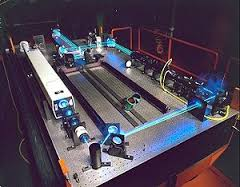
\includegraphics[scale=0.5]{./figs/mesaoptica.jpg}
	\caption{Estupida mesa optica, como te odio.}
	\label{fig:mesaoptica}
\end{figure}


\section{Resultados}

En estas sección se incluyen las tablas de resultados y los gráficos y resultados con una descripción de cómo se obtuvieron. Se muestran los ajustes de curvas, se obtienen los errores por propagación y se discuten los resultados (validez, precisión, interpretación, etc.). Cada figura o tabla debe estar numerada y debe contener una leyenda al pie que permita entenderla sin recurrir al texto completo. La descripción detallada de estas figuras y tablas debe estar incluida también en el texto. Se incluyen las citas a las ecuaciones que se utilizan (que estarán en la introducción).

Ejemplo de una tabla.
Para referenciar una tabla se usa el comando ~\ref{tab:ejemplo}

\begin{table}[H]
\centering
\begin{tabular}[c]{|cc|}% las barras son las lineas verticales. La letra, la alineacion del texto de adentro: l(left), r(right), c(center)
    \hline % linea horizontal
%%    \multicolumn{2}{|c|}{SD Reconstructed Parameters} \\
    %%\hline
    Parámeteros           & Valores \\
    \hline
    En                  & ($1.03 \pm 0.03 \pm 0.04$) $10^{19}$ $eV$      \\
    ($\theta$,$\phi$)   & ($39.5 \pm 0.1$, $108.8 \pm 0.2$) $deg$      \\
    (x,y) Eje           & ($-26.36 \pm 0.01$, $14.58 \pm 0.01$ ) $km$     \\% para cambiar de columna en columna, ponene un signo &
    $S_{450}$           & ($741 \pm 19 (\pm 29)$) $VEM$       \\
    \hline
  \end{tabular}
  \caption{\footnotesize {Pie de tabla de ejemplo.}}
  \label{tab:ejemplo}%etiqueta para despues llamar a la tabla
\end{table}

hola voy a\textbf{ escribir} una letra griega $\varphi$ 
Cualquier cosa que sea una ecuación en el texto la puedo escribir entre signos de \$.

Por ejemplo $X * Y = S_{mu}$. Si quiero llamar a una ecuación que presento aparte, la invoco por su nombre y aparece el numero correspondiente: Ecuación ~\ref{eq:emc}

\begin{equation}
\label{eq:emc}
e = mc^2
\end{equation}

Estaba aburrido y le puse las ecuaciones de Maxwell

\begin{center}
$
\left\{
\begin{array}{cc}
\grad\cdot \mv{D} = 4\pi \rho  & \grad\times\mv{E}=-\frac{1}{c}\dpart{\mv{B}}{t} \\ 
\dive{B}=0 &\rot{B}=\frac{4\pi}{c}\mv{J}+\frac{1}{c}\dpart{\mv{D}}{t} \
\end{array} 
\right.
$
\end{center}

Y las ecuaciones de \textit{Euler-Lagrange} 

$$\dpart{\mathscr{L}}{q_i}(t,q_i.\dot{q_i})-\frac{d}{dt}\dpart{\mathscr{L}}{\dot{q_i}}(t,q_i.\dot{q_i})=0 $$

Están buenisimas.

Luego sigo con el texto 



\begin{figure}[H]
  \centerline{
    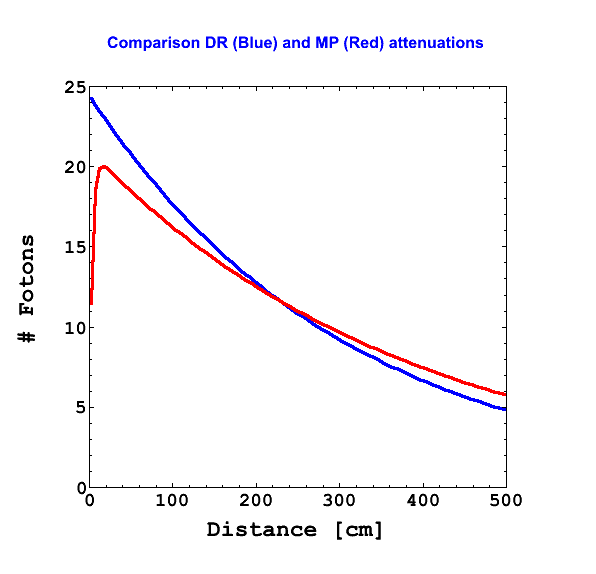
\includegraphics[width=0.5\textwidth]{./figs/Atenuacion.png}}
  \caption{\footnotesize {Ejemplo de pie de figura}}
  \label{fig:atenuacion}
\end{figure}


%------------------------------------------------

\section{Conclusiones y discusi\'on}

Contiene la discusión de cómo, a partir de los resultados, se demuestra aquello que se planteó como objetivo del trabajo tanto en el resumen como en la introducción. En las conclusiones no debe figurar nada que no se haya mencionado anteriormente. 

\section{Agradecimientos}

Se agradece a aquellos que colaboraron en el trabajo, pero cuya participación no amerita la categoría de coautores. Se agradece también a las instituciones que financiaron el proyecto. 

\textbf{Esto asumo que lo vamos a obviar}
%----------------------------------------------------------------------------------------
%	REFERENCE LIST
%----------------------------------------------------------------------------------------

\begin{thebibliography}{99} % Bibliography - this is intentionally simple in this template

\bibitem[1]{PrimerCita}
M. Stalder and M. Schadt
\newblock "Linearly polarized light with axial symmetry generated by liquid-crystal polarization converters" 
\newblock {\em Opt. Lett. 21}, 1948-1950 (1996).
 
\bibitem[2]{SegundaCita}
 J. Goodman
\newblock \underline{\textbf{Introduction to Fourier Optics}} 
\newblock McGraw-Hill, 2nd Edition, New York (1996), pg 254.
 
\textbf{Esto asumo que lo vamos a chamuyar} 
  
\end{thebibliography}

%----------------------------------------------------------------------------------------

\end{multicols}

\end{document}
